\chapter{Machine learning}

The fundamental problem of machine learning can be formalized as follows.

\pr[]{Machine learning problem}{
    Let $X,Y$ be two sets, and $A(X,Y)$ be a set of functions from $X$ to $Y$.
    Assume moreover that we are given a subset $\mathcal F\subset A(X,Y)$ of these functions parametrized over a set $\Theta$, that is
    \begin{equation}
        \mathcal F = \left\{ \phi_\theta \in A(X,Y)\mid \theta\in \Theta \right\}.
    \end{equation}
    Then, given a function $\psi\in A(X,Y)$ the machine learning (ML) problem consists in finding $\hat \theta\in \Theta$ such that
    \begin{equation}
        \psi \approx \phi_{\hat \theta}.
    \end{equation}
    This has to be done using the \emph{available} information about $\psi$.
}

\ex[pointwise-obs]{Linear approximation and pointwise observation}{
    Let $\psi:[0,2\pi]\to \bbR$ be a continuous function (in particular, $\psi\in L^2([0,2\pi]))$).
    
    Consider $\{\phi_i\}_{i=1}^{+\infty}\subset L^2([0,2\pi])\cap C([0,2\pi])$ to be an orthonormal system for $L^2([0,2\pi])$, and for any $N\in \bbN$ let $\Theta = \bbR^N$ and consider
    \begin{equation}
        \mathcal F = \left\{ \phi_\theta = \sum_{i=1}^N \theta_i \phi_i \mid \theta_i\in \bbR^N \right\}
    \end{equation}

    Assume to be given $M$ observations $\{(x_i,y_i)\}_{i=1}^M$ such that
    \begin{equation}
        y_i = \psi(x_i), \qquad i\in \llbracket 1,M\rrbracket.
    \end{equation}
    The task here is to find $\hat \theta\in\Theta$ such that 
    \begin{equation}
        \sum_{i=1}^M \left| \phi_{\hat\theta}(x_i)-y_i \right|^2
        =\min_{\theta} 
        \sum_{i=1}^M \left| \phi_{\theta}(x_i)-y_i \right|^2.
    \end{equation}
}

\ex[]{Finite elements}{
    Let $B_1(0)\subset \bbR^d$ and $\psi : B_1(0)\to \bbR$ be a real-valued function such that $\psi\in H_0^2(B_1(0))$. 
    Then, given independent functions $\{\phi_i\}_{i=1}^N$ we can consider $\Theta=\bbR^N$ and let
    \begin{equation}
        \mathcal F = \left\{ \phi_\theta = \sum_{i=1}^N \theta_i \phi_i \mid \theta_i\in \bbR^N \right\}
    \end{equation}

    A typical situation, and the basis for the \emph{finite element methods}, is to know $f = \Delta \psi$, in which case one looks for $\hat \theta\in \Theta$ such that 
    \begin{equation}
        \|\phi_{\hat\theta}-\psi\|_{L^2} = \min_\theta \|\phi_\theta-\psi\|_{L^2}.
    \end{equation}
}

In modern machine learning one is interested in ``going beyond'' these examples, by considering a nonlinear parametrization of the approximating family $\mcF$. That is, 
\begin{center}
    the map $\theta\mapsto \phi_\theta$ is nonlinear.
\end{center}

In the following we will focus on the problem of data-fitting exoked in Example~\ref{ex:pointwise-obs}, see also Example~\ref{ex:}. This is the following.

\dfn[data-fitting-pb]{Data-fitting problem}{
    Consider the following data:
    \begin{itemize}
        \item A function $\psi:X\to Y$ to approximate, of which only a set of samples $\mfX=\{( x_i,\psi( x_i))\mid i\in \llbracket 1,M\rrbracket\}$ is known;
        \item A set $\mcF = \{\psi_\theta:X\to Y\mid \theta\in \Theta\}$ of possible approximations;
        \item A loss function $\ell : Y\times Y \to \bbR$.
    \end{itemize}
    Then, the data-fitting problem is the following:
    \begin{equation}
        \text{Find } \hat\theta\in\Theta \text{ such that } \hat\theta = \arg\min_{\theta} \frac1N \sum_{(x_i,\hat y_i)\in\mfX} \ell(\phi_\theta(x_i),\hat y_i).
    \end{equation}
}

\begin{figure}
    \centering
    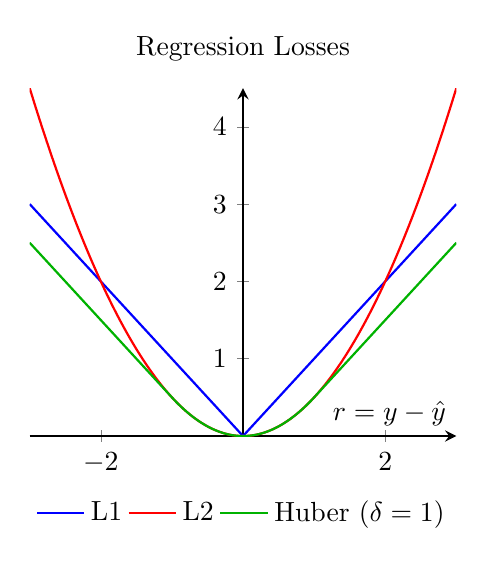
\begin{tikzpicture}
    % ---------------- Left plot: L1, L2, Huber ----------------
    \begin{axis}[
            name=regression,
            at={(0,0)}, anchor=north west,
            xlabel={$r = y - \hat{y}$},
            % ylabel={Loss},
            % grid=major,
            axis lines=middle,
            domain=-3:3,
            samples=200,
            legend style={at={(0.5,-0.15)}, anchor=north, draw=none, legend columns=3},
            width=7cm, height=6cm,
            thick,
            title={Regression Losses}
        ]
        \addplot[blue] {abs(x)};
        \addlegendentry{L1}
        \addplot[red] {0.5*x^2};
        \addlegendentry{L2}
        \addplot[green!70!black] {abs(x) < 1 ? 0.5*x^2 : 1*(abs(x)-0.5*1)};
        \addlegendentry{Huber ($\delta=1$)}
    \end{axis}
\end{tikzpicture}
% ---------------- Right plot: Cross-Entropy ----------------
\hspace{1cm}
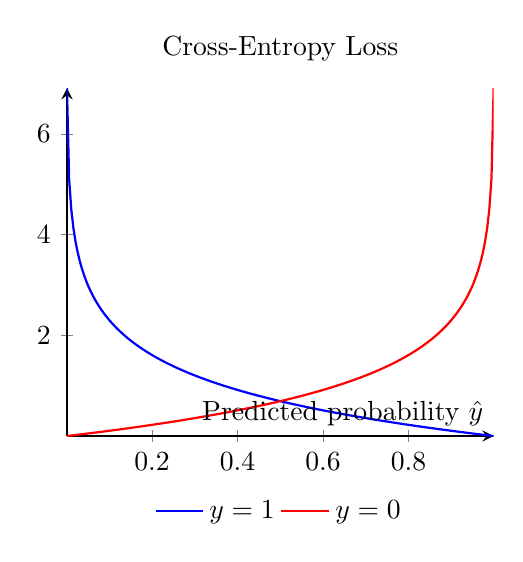
\begin{tikzpicture}
    \begin{axis}[
            xlabel={Predicted probability $\hat{y}$},
            % ylabel={Cross-Entropy Loss},
            % grid=major,
            axis lines=middle,
            domain=0.001:0.999,
            samples=200,
            width=7cm,
            height=6cm,
            thick,
            legend style={at={(0.5,-0.15)}, anchor=north, draw=none, legend columns=2},
            title={Cross-Entropy Loss}
        ]

        % y = 1
        \addplot[blue] {-ln(x)};
        \addlegendentry{$y=1$}

        % y = 0
        \addplot[red] {-ln(1-x)};
        \addlegendentry{$y=0$}
    \end{axis}
\end{tikzpicture}
    \caption{Typical loss functions for $Y=\bbR$ (right) and cross-entropy loss.}
    \label{fig:losses}
\end{figure}

When $Y$ has a vector space structure, it is natural to consider $\ell(y,\hat y)=\ell(r)$ where $r=y-\hat y$ is called the residual.
In this case, typical choices for the loss function are appropriate norms on the space $Y$. 
% 
For example, if $Y\in \bbR^n$ one tyically considers $\ell$ to be the $\ell_1$ or the $\ell_2$. Another common choice is the \emph{Huber error loss}, which ``mixes'' the two. It is defined for $\delta>0$ as
\begin{equation}
    \mfh_\delta(r) = 
    \begin{cases}
        \frac12 \|r\|_2^2, & \text{if }\|r\|_1\le \delta\\
        \delta\left( \|r\|_1 - \frac\delta2 \right)&\text{otherwise.}
    \end{cases}
\end{equation}
See Figure~\ref{fig:losses}, left.

A special mention need to be done in the case for \emph{classification problems}, i.e., problems where the function $\psi$ assigns a discrete label (e.g., cat or dog) to the inputs. In this the relevant values for $\psi$ are $\{0,1\}$, say, but one approximate it with functions taking value in $Y=\bbR$ and interprets values different from $0$ or $1$ as uncertain.
In this case, the most used loss function is the \emph{cross-entropy} function, which is defined by
\begin{equation}
    \ell(y,\hat y) = -\left[ y \log \hat y + (1-y)\log(1-\hat y) \right].
\end{equation}
This function has a probabilistic interpretation and encodes, roughly speaking, the ``surprise'' of seeing $\hat y$ after the model predicted $y$.
See Figure~\ref{fig:losses}, right.





\chapter{Feed-forward neural networks}


In this chapter we introduce and discuss the simplest example of neural network.
These are obtained by concatenating the simplest possible nonlinear operations:
\begin{equation}
    \phi_\theta(x) = \sigma(Wv + b), \qquad \text{where } \theta=(W,b) \in \bbR^{n\times m}\times \bbR^n.
\end{equation}
Here, the function $\sigma:\bbR\to \bbR$ is a nonlinear \emph{activation} function that is assumed to be applied element-wise to the vector $Wx+b$.
Typically activation functions are depicted in Figure~\ref{fig:activations}.

\begin{figure}[b]
    \centering
    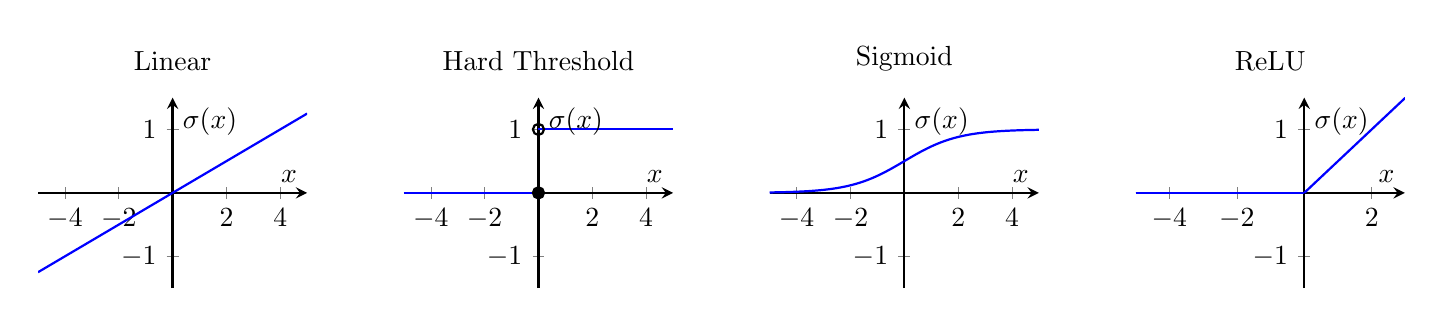
\begin{tikzpicture}[
    every axis/.style={
        width=5cm,
        height=4cm,
        % grid=major,
        axis lines=middle,
        xlabel={$x$},
        ylabel={$\sigma(x)$},
        samples=100,
        domain=-5:5,
        ymin=-1.5, ymax=1.5,
        % xtick={-4,-2,0,2,4},
        ytick={-1,0,1},
        thick
    }
]

% Arrange the four plots in a 1x2 grid
\matrix[column sep=1.2cm, row sep=1.2cm]{

% ---------- Linear ----------
\begin{axis}[title={Linear}]
    \addplot[blue] {x/4}; % scaled down for visibility
\end{axis}
&
% ---------- Hard Threshold ----------
\begin{axis}[title={Hard Threshold}]
    \addplot[blue, domain=-5:0] {0};
    \addplot[blue, domain=0:5] {1};
    \addplot[only marks, mark=*] coordinates {(0,0)};
    \addplot[only marks, mark=o, fill=white] coordinates {(0,1)};
\end{axis}
&
% ---------- Sigmoid ----------
\begin{axis}[title={Sigmoid}]
    \addplot[blue] {1/(1 + exp(-x))};
\end{axis}
&
% ---------- ReLU ----------
\begin{axis}[title={ReLU}]
    \addplot[blue, domain=-5:0] {0};
    \addplot[blue, domain=0:5] {x/2};
\end{axis}
\\
};

\end{tikzpicture}
    \caption{Activation functions}
    \label{fig:activations}
\end{figure}

\dfn[]{One-hidden layer feed-forward ANN}{
    Let $\sigma:\bbR\to \bbR$ be an activation function and let $d_1\in \bbN$.
    A scalar-valued one-hidden layer feed-forward ANN $\psi_\theta:\bbR^d\to \bbR$ is identified by the set of parameters
    \begin{equation}
        \Theta = \left\{ (W_2,W_1,b_1)\in \bbR^{1\times d_1}\times\bbR^{d_1\times d}\times \bbR^{d_1} \right\},
    \end{equation}
    and it reads
    \begin{equation}
        \psi_\theta(x) = W_2\, \sigma(W_1+b_1) = \sum_{j=1}^{d_1} w_{2j} \sigma\left( \sum_{i=1}^{d} w_{ji}x_i + b_{1j} \right).
    \end{equation}

    Here, the \emph{architecture parameters} of the network are
    \begin{itemize}
        \item $d_1\in \bbN$ is the \emph{width} of the hidden layer;
        \item $W_i$ it the \emph{weight} matrix for the $i$-th layer;
        \item $b_1$ is the \emph{bias} of the \first layer.
    \end{itemize}
    }

In Figure~\ref{fig:one-hidden-layer} we present an example of a one-hidden layer feed-forward ANN

\def\layersep{4cm}
\begin{figure}[t]
    \centering
    \begin{adjustbox}{width=.7\textwidth}
        \begin{tikzpicture}[shorten >=1pt,-latex,draw=black!100, node distance=\layersep,auto]

    % INPUT LAYER
    \foreach \name / \y in {1,...,3}
    \node[input neuron] (I-\name) at (0,-2*\y+2.75) {$x_{\name}$};

    % HIDDEN LAYER
    \foreach \name / \y in {1,...,4}
    \node[hidden neuron] (H-\name) at (\layersep,-2*\y+3.5) {$x^2_\name$};

    % OUTPUT LAYER
    \node[output neuron] (O-1) at (2*\layersep,-1.25 cm) {$y$};

    % CONNECTIONS
    % Input -> Hidden
    \foreach \target in {1,...,4}
    \path (I-1) edge node[above] {$w_{1\target}$} (H-\target);

    \foreach \source in {2,...,3}
    \foreach \target in {1,...,4}
    \path[dashed] (I-\source) edge  (H-\target);

    % Hidden -> Output
    \foreach \source in {1,...,4}
    \path (H-\source) edge node[above] {$w_{\source3}$} (O-1);

    % ANNOTATIONS
    \node[annot,above of=H-1, node distance=1.5cm, align=center] (hl) {Hidden layer\\(\second layer)};
    \node[annot,above of=O-1, node distance=2.25cm, align=center] (hl2) {Output layer\\(\third layer)};
    \node[annot,left of=hl, align=center] {Input layer\\(\first layer)};

\end{tikzpicture}

% \begin{tikzpicture}[shorten >=1pt,-latex,draw=black!100, node distance=\layersep,auto]

%     \foreach \name / \y in {1,...,3}
%     \node[input neuron] (I-\name) at (0,-3*\y+2.75) {$x_{\name}$};
%     \path[yshift=1.5cm]
%     node[hidden neuron] (H-1) at (\layersep,-1 cm) {}
%     node[hidden neuron] (Q-1) at (\layersep,-2.5 cm) {}
%     node[hidden neuron] (H-2) at (\layersep,-4 cm) {}
%     node[hidden neuron] (Q-2) at (\layersep,-5.5 cm) {}
%     node[hidden neuron] (H-3) at (\layersep,-7 cm) {}
%     node[hidden neuron] (Q-3) at (\layersep,-8.5 cm) {};
%     \node[hidden neuron] (H2-1) at (2*\layersep,-3*1+2.75) {};
%     \node[hidden neuron] (H2-2) at (2*\layersep,-3*2+2.75) {};
%     \node[hidden neuron] (H2-3) at (2*\layersep,-3*3+2.75) {};
%     \node[output neuron] (H3-1) at (3*\layersep,-3.25 cm) {};
%     \node[annot,right of=H3-1, node distance=1.7cm, align=center] () {};

%     \foreach \y in {1,...,3}
%     \foreach \target in {H,Q}
%     \foreach \source in {1,...,3}
%     \path (I-\source) edge (\target-\y);
%     \foreach \y in {1,...,3}
%     \foreach \source in {H,Q}
%     \foreach \target in {1,...,3}
%     \path (\source-\y) edge (H2-\target);
%     \foreach \y in {1,...,3}
%     \path (H2-\y) edge (H3-1);


%     \node[annot,above of=H-1, node distance=1.5cm, align=center] (hl) {\first hidden layer\\(\second layer)};
%     \node[annot,above of=H2-1, node distance=2.25cm, align=center] (hl2) {\second hidden layer\\(\third layer)};
%     \node[annot,above of=H3-1, node distance=5.25cm, align=center] (hl3) {Output layer\\(\fourth layer)};
%     \node[annot,left of=hl, align=center] {Input layer\\ (\first layer)};

% \end{tikzpicture}
    \end{adjustbox}
    \caption{\label{fig:one-hidden-layer}Graphical illustration of an single hidden layer ANN, yielding a function from $\bbR^3$ to $\bbR$. We only explicited the weights relative to the first variable.}
\end{figure}

The general expression for a feed-forward ANN can then be inferred, see Figure~\ref{fig:deepANN} for a graphical representation.

\dfn[]{Feed-forward fully-connected ANN}{
    Let $\sigma:\bbR\to \bbR$ be an activation function and let $d_1,\ldots, d_N\in \bbN$.
    An $N$-hidden layer feed-forward ANN $\psi_\theta:\bbR^d\to \bbR$ is identified by the set of parameters
    \begin{equation}
        \Theta = \left\{ (W_{N+1},\ldots,W_1,b_1) \mid W_{i}\in\bbR^{d_{i}\times d_{i-1}}, \, b_i\in \bbR^{d_i} \right\},
    \end{equation}
    where we let $d_0=d$ and $d_{N+1}=n$. 
    The corresponding function is then
    \begin{equation}
        \label{eq:ANN}
        \phi\theta(x) = \psi^{N+1} \circ \psi^N \circ\cdots\psi^1(x),
    \end{equation}
    where 
    \begin{gather}
        \phi^{i}: x_{i-1} \in \bbR^{d_{i-1}}\mapsto \sigma(W_i x_{i-1}+b_i)\in \bbR^{d_i}, \qquad \forall i\in \llbracket 1,N\rrbracket\\
        \phi^{N+1}: x_{N} \in \bbR^{d_{N}}\mapsto W_N x_{N}\in \bbR.
    \end{gather}

    Here, the \emph{architecture parameters} of the network are
    \begin{itemize}
        \item $d_i\in \bbN$ is the \emph{width} of the \nth{i} hidden layer;
        \item $W_i$ it the \emph{weight} matrix for the \nth{i} layer;
        \item $b_i$ is the \emph{bias} of the \nth{i} layer.
    \end{itemize}
}

\begin{figure}
    \centering
	% \hspace{-2cm}
    \begin{adjustbox}{width=.9\textwidth}
         \begin{tikzpicture}[shorten >=0pt,-latex,draw=black!100, node distance=\layersep,auto, scale=0.92]
     \def\layersep{2.9cm}
     \def\neuronsep{1.8cm}
     \def\ninput{3}
     \def\nhidden{5}
     \def\noutput{3}
 
     \tikzmath{
         \ninputl=\ninput-1;
         \nhiddenl=\nhidden-1;
         \noutputl=\noutput-1;
         \nmax=max(\ninput,\nhidden,\noutput);
     }
 
     \foreach \inode in {1,...,\ninputl}
     \node[input neuron] (I-\inode) at (0,.5*\ninput*\neuronsep-\inode*\neuronsep+\neuronsep) {$\inode$};
     \node (I-dots) at (0,.5*\ninput*\neuronsep-\ninputl*\neuronsep) {$\vdots$};
     \node[input neuron] (I-\ninput) at (0,.5*\ninput*\neuronsep-\ninput*\neuronsep) {$l_0$};
 
     \foreach \inode in {1,...,\nhiddenl}
     \node[hidden neuron] (H1-\inode) at (\layersep,.5*\nhidden*\neuronsep-\inode*\neuronsep+\neuronsep) {$\inode$};
     \node (H1-dots) at (\layersep,.5*\nhidden*\neuronsep-\nhiddenl*\neuronsep) {$\vdots$};
     \node[hidden neuron] (H1-\nhidden) at (\layersep,.5*\nhidden*\neuronsep-\nhidden*\neuronsep) {$x_1$};
 
     \foreach \inode in {1,...,\nhiddenl}
     \node[hidden neuron] (H2-\inode) at (2*\layersep,.5*\nhidden*\neuronsep-\inode*\neuronsep+\neuronsep) {$\inode$};
     \node (H2-dots) at (2*\layersep,.5*\nhidden*\neuronsep-\nhiddenl*\neuronsep) {$\vdots$};
     \node[hidden neuron] (H2-\nhidden) at (2*\layersep,.5*\nhidden*\neuronsep-\nhidden*\neuronsep) {$x_2$};
 
     \foreach \inode in {1,...,\nhiddenl}
     \node (Hdots-\inode) at (3*\layersep,.5*\nhidden*\neuronsep-\inode*\neuronsep+\neuronsep) {$\cdots$};
     \node (Hdots-dots) at (3*\layersep,.5*\nhidden*\neuronsep-\nhiddenl*\neuronsep) {$\ddots$};
     \node (Hdots-\nhidden) at (3*\layersep,.5*\nhidden*\neuronsep-\nhidden*\neuronsep) {$\cdots$};
 
     \foreach \inode in {1,...,\nhiddenl}
     \node[hidden neuron] (H3-\inode) at (4*\layersep,.5*\nhidden*\neuronsep-\inode*\neuronsep+\neuronsep) {$\inode$};
     \node (H3-dots) at (4*\layersep,.5*\nhidden*\neuronsep-\nhiddenl*\neuronsep) {$\vdots$};
     \node[hidden neuron] (H3-\nhidden) at (4*\layersep,.5*\nhidden*\neuronsep-\nhidden*\neuronsep) {$x_{N}$};
 
     \foreach \inode in {1,...,\noutputl}
     \node[output neuron] (O-\inode) at (5*\layersep,.5*\noutput*\neuronsep-\inode*\neuronsep+\neuronsep) {$\inode$};
     \node (O-dots) at (5*\layersep,.5*\noutput*\neuronsep-\noutputl*\neuronsep) {$\vdots$};
     \node[output neuron] (O-\noutput) at (5*\layersep,.5*\noutput*\neuronsep-\noutput*\neuronsep) {$x_{N+1}$};
 
     \foreach \inode in {1,...,\ninput}
     \foreach \hnode in {1,...,\nhidden}
     \path (I-\inode) edge (H1-\hnode);
 
     \foreach \inode in {1,...,\nhidden}
     \foreach \hnode in {1,...,\nhidden}
     \path (H1-\inode) edge (H2-\hnode);
 
     \foreach \inode in {1,...,\nhidden}
     \foreach \hnode in {1,...,\nhidden}
     \path (H2-\inode) edge [-] (Hdots-\hnode);
 
     \foreach \inode in {1,...,\nhidden}
     \foreach \hnode in {1,...,\nhidden}
     \path (Hdots-\inode) edge (H3-\hnode);
 
     \foreach \inode in {1,...,\nhidden}
     \foreach \hnode in {1,...,\noutput}
     \path (H3-\inode) edge (O-\hnode);
 
     \node[annot] (input) at (0,.5*\nmax*\neuronsep+.5*\neuronsep) {Input layer\\(\first layer)};
     \node[annot] (hidden1) at (\layersep,.5*\nmax*\neuronsep+.5*\neuronsep) {\first hidden layer\\(\second layer)};
     \node[annot] (hidden2) at (2*\layersep,.5*\nmax*\neuronsep+.5*\neuronsep) {\second hidden layer\\(\third layer)};
     \node[annot] (dots) at (3*\layersep,.5*\nmax*\neuronsep+.5*\neuronsep) {$\cdots$};
     \node[annot] (hidden3) at (4*\layersep,.5*\nmax*\neuronsep+.5*\neuronsep) {\nth{$N$} hidden layer\\(\nth{$N+1$} layer)};
     \node[annot] (output) at (5*\layersep,.5*\nmax*\neuronsep+.5*\neuronsep) {Output layer\\(\nth{$(N+2)$} layer)};
 \end{tikzpicture}
    \end{adjustbox}
\caption{\label{fig:deepANN}Graphical illustration of a fully-connected feedforward ANN consisting of
$N+2\in\bbN$ affine transformations (i.e., consisting of $N+1$ layers: one input layer, $N$ hidden layers, and one output layer). Image from \cite{jentzenMathematicalIntroductionDeep2023}.}
% with $l_-1\in\bbN$ neurons on the input layer (i.e., with $l_0$-dimensional input layer), with
% $l_0\in\bbN$ neurons on the \first hidden layer (i.e., with $l_1$-dimensional \first hidden layer),
% with $l_1\in\bbN$ neurons on the \second hidden layer (i.e., with $l_2$-dimensional \second hidden layer),
% $\dots$, with $l_{L-2}$ neurons on the \nth{$(L-1)$} hidden layer (i.e., with $(l_{L-1})$-dimensional \nth{$(L-1)$} hidden layer),
% and with $l_L$ neurons in the output layer (i.e., with $l_L$-dimensional output layer). Image from \cite{jentzenMathematicalIntroductionDeep2023}.}
\end{figure}

\section{Learning and backpropagation}

Once a loss function has been chosen, the data-fitting problem of Definition~\ref{def:data-fitting-pb} can be solved using the algorithms presented in Chapter~\ref{chp:numerical-algo}, along with their various extensions.  
All of these algorithms, however, require the computation of the gradient of the loss function, which in turn involves differentiating the function $\phi_\theta$ from \eqref{eq:ANN}.  
This task is particularly challenging because $\phi_\theta$ is defined as a composition of many functions. Even in the simplified case where $\sigma$ is the identity (i.e., $\sigma(x) = x$), expanding \eqref{eq:ANN} explicitly leads to a sum with an order of $d_1 \times \dots \times d_N$ terms.  
In contemporary neural networks, the layer dimensions $d_1, \dots, d_N$ are so large that explicitly computing such a sum is completely infeasible, which is why efficient methods like backpropagation are essential.


\chapter{Residual neural networks, neural ODEs and control}